\documentclass[a4paper,11pt]{article}
\usepackage{graphicx,listings,float,epstopdf,geometry, caption,subcaption, placeins}
\setcounter{tocdepth}{2}
\usepackage[dutch]{babel}

\geometry{
	includeheadfoot,
	margin=2.54cm
}

\begin{document}
\subsection{Schieten met het lasergeweer}
Men kan opmerken uit figuur \ref{fig:UI} dat de schietrichting niet meteen duidelijk uit de interface wordt. Immers, het vizier wordt niet op het scherm, op het zelfde punt afgebeeld. Echter het vizier is eenvoudig mee te richten, daarom wordt bij het schieten een laser afgevuurd vanuit het wapen naar het punt waar de vizier op gericht staat. Dit is te zien in figuur \ref{fig:COL}.
 
\begin{figure}[h]
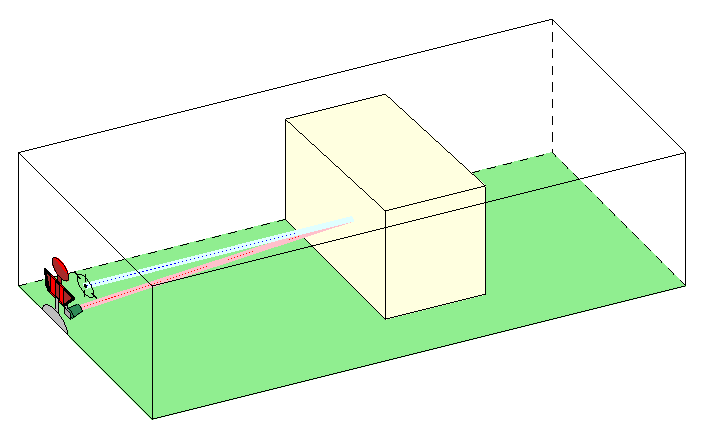
\includegraphics[width=\textwidth]{Graphics/Collision.eps}
\caption{Een voorbeeld van het schieten van je geweer}
\label{fig:COL}
\end{figure}


Een ander probleem wat voor kan komen, is dat het vizier een bepaald punt aanwijst, maar dat de laser geen schot kan afvuren naar dit punt omdat een object voor dit punt staat. Er zijn dan twee manieren om dit op te lossen, men kan zeggen dat de laser altijd het punt van de vizier raakt. Dit is makkelijker te implementeren, aangezien we maar \'e\'en keer hoeven te bepalen waar een lijn een object. Dit is te zien in figuur \ref{fig:COL2} Een andere oplossing is om de laser in de richting van het punt een schot af te vuren en als er een object in de weg staat, dit object te raken. Dit is natuurlijk realistischer maar minder makkelijk te implementeren. Dit is te zien in figuur \ref{fig:COL3}. In eerste instantie kiezen wij voor de eerste methode. Echter, bij een tijdoverschot, kunnen wij de tweede manier implementeren.
\FloatBarrier
\begin{figure}[h]
\begin{subfigure}{\textwidth}
\centering
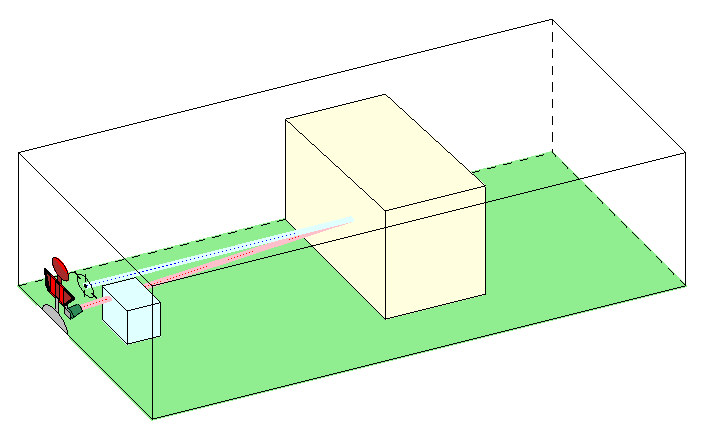
\includegraphics[width=0.7\textwidth]{Graphics/Collision2.eps}
\caption{De laser komt altijd aan op het punt aangewezen door het vizier}
\label{fig:COL2}
\end{subfigure}\\
\begin{subfigure}{\textwidth}
\centering
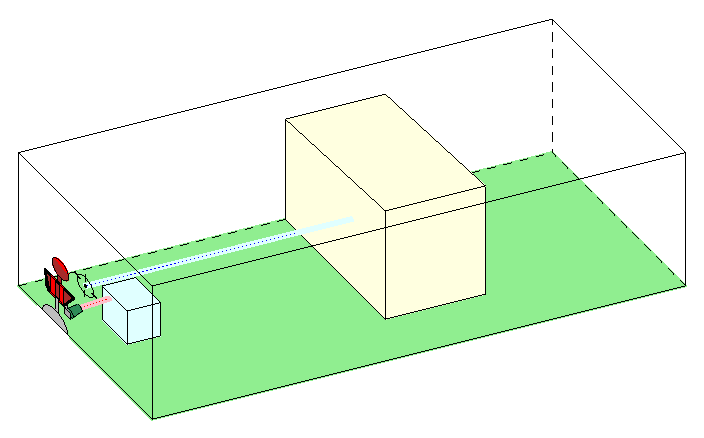
\includegraphics[width=0.7\textwidth]{Graphics/Collision3.eps}
\caption{De laser stopt zodra hij een ander object raakt}
\label{fig:COL3}
\end{subfigure}
\end{figure}
\end{document}
